%%% -*- TeX-engine: xetex -*-
\documentclass{beamer}

% for themes, etc.
\usepackage{times}  % fonts are up to you
\usepackage{graphicx}
\usepackage{color}
\mode<presentation>
{
 \usetheme{Warsaw}
 \useoutertheme{infolines}
 \usecolortheme{whale}
 \setbeamertemplate{navigation symbols}{}
}
\usepackage{xeCJK}
\setCJKmainfont{WenQuanYi Micro Hei}

\title{基于翻译技术的流量调度}
\author{王文鑫}
\date{2016年1月5日}
\AtBeginSection[]
{
  \begin{frame}<beamer> 
    \tableofcontents[currentsection]
  \end{frame}
}

\begin{document}

\begin{frame}
  \titlepage
\end{frame}

\section{背景介绍}
\subsection{MAP-T}

\begin{frame}
  \frametitle{MAP-T}

  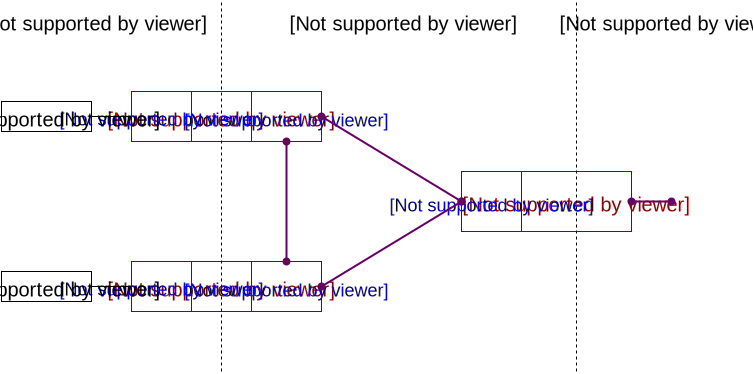
\includegraphics[width=\textwidth]{figs/MAP-T.pdf}  
  \vspace{1.5em}
  使用IPv6网络,将内部IPv4网络与公共IPv4网络相连
\end{frame}

\begin{frame}
  \frametitle{Mapping of Address and Port Using (NAT64) Translation}

  \begin{block}{做法}
    \begin{itemize}
    \item 使用NAT64,在IPv6网络上传输IPv4数据包
    \item 使用固定的端口划分和分配共享全局地址
    \item 每个CPE获取一段全局地址的端口,进行私有IPv4地址到全局IPv4地址的端口映射
    \item 使用一个特定的IPv6前缀翻译进出口的数据包,通过路由引向BR
    \end{itemize}
  \end{block}

  \begin{block}{优点}
    \begin{itemize}
    \item 实现对全局地址的共享
    \item 私有到全局地址的映射状态分布在各个CPE上
    \item 一级翻译器(BR)无需维护每个连接的映射状态
    \end{itemize}
  \end{block}

\end{frame}

\begin{frame}
  \frametitle{Mapping of Address and Port Using (NAT64) Translation}

  \includegraphics[width=\textwidth]{figs/MAP-T-details.png}  
\end{frame}

\subsection{高复用比带来的问题}

\begin{frame}
  \frametitle{高复用比带来的问题}

  \begin{itemize}
  \item 每个CPE可以用来进行映射的端口数有限
  \item 一旦这些端口耗尽,就无法为新连接提供映射
  \end{itemize}
\end{frame}

\begin{frame}
  \frametitle{解决方法}
  \includegraphics[width=\textwidth]{figs/MAP-T-DS-Lite.pdf}  

  转而使用粒度更细、复用比更高的NAT,如DS-Lite
\end{frame}

\section{研究目标}
\subsection{研究目标}
\begin{frame}
  \frametitle{研究目标}

  \includegraphics[width=\textwidth]{figs/MAP-T-Multiple-DS-Lite.pdf}  
  \vspace{1.5em}
  引入多个有状态的一级翻译机,在这些翻译机间调度超出复用比额度的流量
\end{frame}

\begin{frame}
  \frametitle{目的}
  \begin{itemize}
  \item 负载均衡
  \item 容错
  \item 特定路由策略
    \begin{itemize}
    \item 根据目的地,选择在某个运营商出口的翻译机
    \item 为某些网络应用单独分配翻译机
    \end{itemize}
  \item 调度算法也许可以用于多个MAP-T一级翻译机的场景
  \end{itemize}
\end{frame}

\subsection{模型}
\begin{frame}
  \frametitle{模型}
  \includegraphics[height=8em]{figs/CPEs-BRs.pdf}  
\end{frame}

\section{研究路线}
\subsection{工作划分}

\begin{frame}
  \frametitle{工作划分}
  \begin{block}{算法}
    \begin{itemize}
    \item 选择算法:决定某个数据包使用的翻译器
      \begin{itemize}
      \item 在CPE上完成
      \end{itemize}
    \item 分配算法:决定某个CPE可以使用的翻译器集合
    \end{itemize}
  \end{block}
\end{frame}

\subsection{选择算法}

\begin{frame}
  \frametitle{选择算法:决定某个数据包使用的翻译器}
  \begin{block}{类比4层负载均衡器}
    \begin{itemize}
    \item 轮询
    \item 最小连接数
    \item 加权
      \begin{itemize}
      \item 轮询
      \item 最小连接数
      \end{itemize}
    \item 地址哈希
      \begin{itemize}
      \item 需要处理地址非均匀分布的情况
      \end{itemize}
    \end{itemize}
  \end{block}
\end{frame}

\begin{frame}
  \frametitle{选择算法}
  \begin{block}{特定的路由策略}
  \begin{itemize}
  \item 将有特定目的的一级翻译器分成不同的策略组
    \begin{itemize}
    \item 电信组、优库组……默认组
    \end{itemize}
  \item 每个流匹配到一个策略组内
  \item 若组内有多个翻译器,则继续负载均衡
  \end{itemize}
  \end{block}
\end{frame}

\begin{frame}
  \frametitle{选择算法}
  \begin{block}{难点}
    \begin{itemize}
    \item 有效地在分配到的翻译器中分配负载
    \item 结合分配算法,使得各翻译器间的负载达到均衡
    \item 对于有连接的传输协议(TCP),保证某个流的所以包通过相同的翻译器
    \end{itemize}
  \end{block}
\end{frame}

\subsection{分配算法}

\begin{frame}
  \frametitle{分配算法:CPE共享所有翻译器}
  \begin{itemize}
  \item 依赖CPE的选择算法进行负载均衡
  \item 可以在CPE间协调
  \item 无法根据一级翻译器的状态进行调整
  \end{itemize}
\end{frame}

\begin{frame}
  \frametitle{分配算法:在CPE间静态分配翻译器}
  \begin{itemize}
  \item 在配置CPE时指定可以使用的翻译器
  \item 无法使用其它CPE得到的翻译器
    \begin{itemize}
    \item 即便它们是空闲的
    \item 即便本CPE得到的翻译器出错
    \end{itemize}
  \end{itemize}
\end{frame}

\begin{frame}
  \frametitle{分配算法:在CPE间动态分配翻译器}
  \begin{block}{引入中心控制器}
    \begin{itemize}
    \item 获取各个一级翻译器的状态
    \item 为各个CPE分配翻译器
    \item 当翻译器的负载/状态发生变化时,重新分配
    \end{itemize}
  \end{block}
\end{frame}

\begin{frame}
  \frametitle{分配算法:在CPE间动态分配翻译器}
  \begin{block}{中心控制器的好处}
    \begin{itemize}
    \item 类似于SDN中,控制器掌握所有路由器的状态,统一控制路由走向
    \item 控制器掌握所有翻译器的状态,对出口流量进行统一调度
    \item 否则,由各个CPE单独获取翻译器状态,并协调分配
      \begin{itemize}
      \item 效率低,收敛慢
      \end{itemize}
    \end{itemize}
  \end{block}
\end{frame}

\begin{frame}
  \frametitle{分配算法:难点}
  \begin{itemize}
  \item 结合选择算法,使得无论整体负载稳定与否,各翻译器间的负载尽量达到均衡
  \item 在平稳状态下,各翻译器的负载应当较为稳定,不应抖动
  \item 对于有连接的传输协议(TCP),需要保证某个流的所有包通过相同的翻译器
    \begin{itemize}
    \item 即便某个CPE分配到的翻译器集合发生变化,当前未结束的流的路由应该保持不变
    \end{itemize}
  \end{itemize}
\end{frame}

\section{参考文献}
\begin{frame}
  \frametitle{参考文献}
  \begin{itemize}
  \item Understanding CSM Load Balancing Algorithms
  \end{itemize}
\end{frame}
\end{document}
